\documentclass{article}

\usepackage{amsmath, amssymb}
\usepackage{fullpage}
\usepackage{listings}% http://ctan.org/pkg/listings
\lstset{
  basicstyle=\ttfamily,
  mathescape
}
\usepackage{times}
\usepackage{url}
\usepackage[colorlinks=true, linkcolor=blue,]{hyperref}
\usepackage{xcolor}
\usepackage{tikz,subfig}
\usetikzlibrary[topaths]
%\tikzset{%
%  do path picture/.style={%
%    path picture={%
%      \pgfpointdiff{\pgfpointanchor{path picture bounding box}{south west}}%
%        {\pgfpointanchor{path picture bounding box}{north east}}%
%      \pgfgetlastxy\x\y%
%      \tikzset{x=\x/2,y=\y/2}%
%      #1
%    }
%  },
%  cross/.style={do path picture={    
%    %\draw [line cap=round] (-1,-1) -- (1,1) (-1,1) -- (1,-1);
%    \draw [line cap=round] (#1.north east) -- (#1.south west) (#1.north west) -- (#1.south east);
%  }},
%}

\newcommand{\Z}{\mathbb{Z}}
\newcommand{\dv}{{\mathrm{div}}}
\newcommand{\md}{{\mathrm{mod}}}
\newcommand{\lcm}{{\mathrm{lcm}}}

\date{January 15, 2018}
\title{The 3\textsuperscript{rd} Problem Set}

\begin{document}
\maketitle
\section*{Pre-requisites}
You should do the followings
\begin{enumerate}
\item On a separate and clean paper,  you need to describe your own strategy to solve the problems below, and 
	to justify why your strategy is effective while handling each problem
\item On a new clean paper, transform your strategy into an algorithm, using your own form to express algorithms.
	Further, you need to analyze the total running steps of your algorithm and the required memory amount to finish your algorithm.
	Then express the total costs using Big-O notation.
\item Use the \texttt{Code ocean} (\url{https://codeocean.com}) platform; if necessary, you may invite me using my email address 
\texttt{lightsun.kim@gmail.com}.
\item Time limits for each problem
\begin{itemize}
\item Problem \#1: Within 5 hours
\item Problem \#2: Within 3 hours
\item Problem \#3: Within 3 hours
\end{itemize}
Then you need to prepare two answer codes; one is a C code that you have made within each time limit, and the
other is a C code augmented and fixed from the original code later.
\end{enumerate}

\newpage

\section{Problem \#1}

In this problem, we consider the max subarray problem. 
Here we are given an integer  array $A$ and asked to find the subarray
whose elements have the largest sum. More formally,
given array $A=[a_1:a_n]=[a_1,a_2,\ldots,a_n]$, you are requested to find indices 
$\alpha$ and $\beta$ that maximize the sum
\begin{equation*}
S_{\alpha:\beta}=a_{\alpha}+a_{\alpha+1}+\cdots+a_{\beta}=\sum_{\alpha\leq i\leq \beta} a_i.
\end{equation*}
You should note that each $a_i$ is an integer, and thus it could have a positive, negative, or zero value.

Throughout Problem \#1, we let $A[0]=0$, and let $A[\alpha:\beta]$ denote the sequence of elements of $A$
from index $\alpha$ to $\beta(0\leq \alpha\leq\beta\leq n)$. 
To wrap up, the max subarray problem consists of finding the sequence $A[\alpha:\beta]$ that 
maximizes $S_{\alpha:\beta}$, the sum of its values.
Then such a max sum is called the max subarray sum of array $A$.

For example, given an array $A[1:11]=[-2,-4,3,-1,5, 6,-7,-2,4,-3,2]$,
the max subarray is $A[3:6]$ and the max subarray sum is $S_{3,6}=13$. 

For this problem, a naive solution is the following algorithm, named \textsf{MaxsubCubic}:
\begin{table}[h]
\centering
\begin{tabular}{lrlllll}\hline
\multicolumn{7}{l}{\textsf{Algorithm} MaxsubCubic} \\ \hline
\multicolumn{7}{l}{INPUT: An $n$-element integer array $A$ whose elements are indexed from $1$ to $n$.}\\
\multicolumn{7}{l}{OUTPUT: The max subarray sum $S_{\alpha:\beta}$ and its pair of indices $(\alpha,\beta)$ of $A[\alpha:\beta]$.} \\ 
&1. & \multicolumn{5}{l}{$\text{max}\gets 0$}\\
%&2. &  & \multicolumn{4}{l}{$d\gets a,s\gets 1,t\gets 0$}\\
%&3. &  & \multicolumn{4}{l}{\texttt{return} $(d,s,t)$}\\
&2. & \multicolumn{5}{l}{\textbf{for} $j\gets 1$ \textbf{to} $n$}\\
%&5. & \multicolumn{5}{l}{$i\gets 1$}\\
%&6. & \multicolumn{5}{l}{\texttt{do}}\\
&  3. &  & \multicolumn{4}{l}{\textbf{for} $k\gets j$ \textbf{to} $n$}\\
&  4. &  & &\multicolumn{3}{l}{$S\gets 0$}\\
&  5. &  & & \multicolumn{3}{l}{\textbf{for} \underline{\hspace{5cm}}\hfill(1)}\\
&  6. &  & & & \multicolumn{2}{l}{$S\gets $\underline{\hspace{5cm}}\hfill(2)}\\
&  7. &  & & \multicolumn{3}{l}{\textbf{if} $S>\text{max}$ \textbf{then}}\\
&8. & & & &\multicolumn{2}{l}{$\text{max}\gets S$}\\
&9. & & & &\multicolumn{2}{l}{$(\alpha,\beta)\gets (j,k)$}\\
%& 13. & \multicolumn{5}{l}{$d\gets r_{i-1},s\gets s_{i-1},t\gets t_{i-1}$}\\ 
&10. &  \multicolumn{5}{l}{\textbf{return} $\text{max},(\alpha,\beta)$}\\\hline
\end{tabular}
\end{table}


Here you can easily see that thanks to for-loop in Line 5, 
the running time of the \textsf{MaxsubCubic} is $O(n^3)$. 
Therefore, this complexity is really bad, especially when the index $n$ is huge.
Now, your main mission in this problem is to find a way to improve this algorithm so that 
its running time complexity has only $O(n)$.






\bigskip
\noindent\textbf{Language requirements. }%
During tackling this problem, you should follow the programming rules:
\begin{itemize}
\item You should use an ANSI C programming language whose source code can run on \texttt{Code ocean} platform. 
\item Function naming: Begin with the lower character, and every parameters are strong-typed variables (i.e., do not use \texttt{void} typed variables).
	All functions should have a single return value; thus even if a function will return no values; you should provide \texttt{return} keyword.
\item Variable naming: Begin with a type-discriminating prefix. For example, if a variable name is for an age and is with an integer type,
	you need to declare the variable as \texttt{int iAge;}  Especially for string-type variables you are strongly recommended to use the prefix \texttt{sz}.
	For example, if a variable name is for a name, then \texttt{szName} is a preferable choice.
\end{itemize}

\bigskip
\noindent\textbf{Input format.} %
The input is given a text-format file, named \texttt{input.txt} and all strings are separated by commas.
You should take as input integers $a_i$ with $i\geq 1$ and construct an integer array $A[1:n]=[a_1,a_2,\ldots,a_n]$.
Note that the input file does not include the size of the array $A$; thus the input file is in form as follows:
\begin{lstlisting}[backgroundcolor=\color{yellow!40}]
$a_1,a_2,\ldots,a_n$
\end{lstlisting}



\bigskip
\noindent\textbf{Output format.} %
The output should be given as a text-format file, named \texttt{outputc.txt}, \texttt{outputq.txt}, or \texttt{outputl.txt}.
The output file writes (1) the max subarray $A[\alpha:\beta]$, (2) its sum $S_{\alpha:\beta}$, and (3) the execution time as follows:

\begin{lstlisting}[backgroundcolor=\color{yellow!40}]
***************************************
By Maxsub{Cubic or Quadratic or Linear}
***************************************
$\ast\ast$ The max subarray $\ast\ast$
$A[\alpha:\beta]$=$[a_{\alpha},a_{\alpha+1},\ldots,a_{\beta}]$

$\ast\ast$ Its sum $\ast\ast$
$S[\alpha:\beta]$=

The total execution time: ______ sec
\end{lstlisting}

You should provide three programs: The first program is your  C code of \textsf{MaxsubCubic}
that completes (1) and (2) of Line 5 and 6 in the algorithm above. Then you need to improve the algorithm 
so that it has the running time $O(n^2)$; this improved algorithm is named \textsf{MaxsubQuadratic}.
Finally you should enhance your \textsf{MaxsubQuadratic} algorithm so that it has the running time $O(n)$ whose name 
is given by \textsf{MaxsubLinear}.
Moreover, your codes should provide the execution times of all your C programs using described in Problem \#2 of the first problem set.


\newpage
\section{Problem \#2}
Let $\Z$ be the set of integers, and let $a,b\in\Z$.
We say that $a$ divides $b$ if there exists an integer $k$ such that $b=ak$ and 
we write it as $a|b$.
Given two integers $a,b$, a common divisor $d$ of $a$ and $b$ is $d|a$ and $d|b$;
moreover we call such a $d$ the greatest common divisor (GCD) of $a$ and $b$ if
$d\geq 0$ and all other common divisors of $a$ and $b$ divide $d$.
For $a,b\in\Z$, a common multiple of $a$ and $b$ is an integer $m$ such that $a|m$ and $b|m$;
moreover, such an $m$ is the least common multiple (LCM) of $a$ and $b$ if
$m\geq 0$ and $m$ divides all other common multiples of $a$ and $b$.


Let $S=\{a_1,a_2,\ldots,a_n\}\subset\Z$ for some $n>1$. Let $\ell={n\choose 2}=\frac{n!}{2!(n-2)!}$.
For notational convenience, we use the following symbols
\begin{itemize}
\item For each of  two distinct elements $a,b\in S$, we have the GCD of $a$ and $b$; we write each GCD as $d_i=\gcd(a,b)(1\leq i\leq \ell)$. 
\item Similarly, for each of  two distinct elements $a,b\in S$, we have the LCM of $a$ and $b$; we write each LCM as $m_i=\lcm(a,b)(1\leq i\leq \ell)$.
\end{itemize}

In this problem, your mission is to develop a C code to find two pairs of values $X:=(a,b)$ and $Y:=(a^\ast,b^\ast)$ so that
when $d=\gcd(a,b)$ and $m^\ast=\lcm(a^\ast,b^\ast)$ for some $a,b,a^\ast,b^\ast\in S$, 
one has $d=\displaystyle\min_{1\leq i\leq \ell}d_i$ and $m^\ast=\displaystyle\max_{1\leq i\leq \ell}m_i$.
 
\bigskip
\noindent\textbf{Input format.} %
The input is given a text-format file, named \texttt{input.txt} and all strings are separated by commas.
\begin{lstlisting}[backgroundcolor=\color{yellow!40}]
$n$
{$a_1$, $a_2$, $\ldots$, $a_n$} 
\end{lstlisting}
where $n$ is the number of elements is a set $S$.
Namely, the set $S=\{a_1,a_2,\ldots,a_n|a_i\in\Z\}$ and an integer $n\geq 10$.
We assume that every integer has the length of less than or equal to 32 bits, but note that $S$ may have a negative element.
One way to have such a set is (1) to randomly generate $n$ integers, (2) to choose a positive integer $k<n$ randomly,
(3) to create a set of random indices $J=\{i_1,i_2,\ldots,i_k\}$, and (4) to set $a_{i_j}$ into $-a_{i_j}$ for each $j\in J$.

 
\bigskip
\noindent\textbf{Output format.} %
The output should be given as a text-format file, named \texttt{output.txt}.
The output file writes the resulting  values $d$ and $d^\ast$ along with the corresponding pairs $(a,b)$ and $(a^\ast,b^\ast)$ such that
$d=\gcd(a,b)$ and $m^\ast=\lcm(a^\ast,b^\ast)$ under the condition described as above.
 
\begin{lstlisting}[backgroundcolor=\color{yellow!40}]
S={$a_1$, $a_2$, $\ldots$, $a_n$}

$\ast\ast$ The smallest GCD $\ast\ast$
$d$=gcd($a$, $b$)

$\ast\ast$ The largest LCM $\ast\ast$
$m^\ast$=lcm($a^\ast$, $b^\ast$)
\end{lstlisting}

%
% 
\newpage
\section{Problem \#3}

The Josephus problem is mentioned in  Exercise \textbf{A-2.1} of the textbook~\cite{GT15}, but 
the  problem in its original form goes long back to the Roman historian Flavius Josephus~\cite{Jos27}.

There has been known an interesting history   as follows:
In the Romano-Jewish conflict of   67 A.D., finally the Romans occupied the town ``Jotapata'' which \textit{Josephus} was ruling.
During the last battle against Rome's army,  he and   $40$ companions escaped and trapped in a cave. 
They have fallen the fear of death, and so they decided to kill themselves at  all time.
At this point of decision,   Josephus and a friend did not agree with that proposal, of course,
  but were afraid to stay in their opposition.
Thus they (i.e., Josephus and the friend) suggested that they should arrange them in a circle and that counting around the circle  
in the same sense all the time,   every third man should be killed until there was only one survivor who would kill himself.  
By choosing the position $31$   and $16$   in the circle Josephus
and his companion saved their lives.\footnote{How did Josephus become  Roman historian? How survived? Why historian of all choices?; Quite interesting :-)}


Historically, it is not clear that he suggested such an idea to take care about only his own survival.
In other words, no one knows the truth of the day among them.
Today, one apparent thing is  that a quite interesting problem, called the Josephus problem, has been introduced.


We now describe  the Josephus problem  more formally and generally. 
There is a group of $n$ people ($n=41$ in the case of Josephus and his 40 companions) and 
let each person  (say $u_i,1\leq i\leq n$) stand in a node of a circle, numbered consecutively clockwise from 1 to $n$ as follows. 

\begin{figure}[h]
\centering
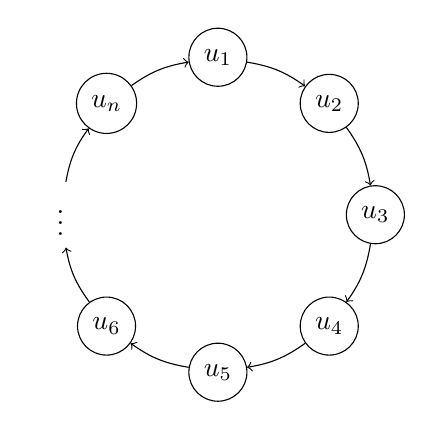
\begin{tikzpicture} 
\node[circle,draw] (u3) at (0:2) {$u_3$};
\node[circle,draw] (u2) at (45:2) {$u_2$};
\node[circle,draw] (u1) at (90:2) {$u_1$};
\node[circle,draw] (u8) at (135:2) {$u_n$};
\node[circle,draw=none] (u7) at (180:2) {$\vdots$};
\node[circle,draw] (u6) at (225:2) {$u_6$};
\node[circle,draw] (u5) at (270:2) {$u_5$};
\node[circle,draw] (u4) at (315:2) {$u_4$};
\path (u1) edge [->,bend left=13] (u2);
\path (u2) edge [->,bend left=13] (u3);
\path (u3) edge [->,bend left=13] (u4);
\path (u4) edge [->,bend left=13] (u5);
\path (u5) edge [->,bend left=13] (u6);
\path (u6) edge [->,bend left=13] (u7);
\path (u7) edge [->,bend left=13] (u8);
\path (u8) edge [->,bend left=13] (u1);
\end{tikzpicture}
\end{figure}
Then staring with  person no. 1 (i.e., $u_1$), it kills $u_2$, $u_3$ kills $u_4$, $u_5$ kills $u_6$, and proceeding clockwise in the same manner.
We continue the process with the remaining people; that is, $u_1$ kills $u_3$, $u_5$ kills $u_7$, and proceeding clockwise.
We will continue this process until only one person survives. For example, suppose that $n=8$.
\begin{figure}[h]
\centering
\subfloat[][Initial]{\label{f1}
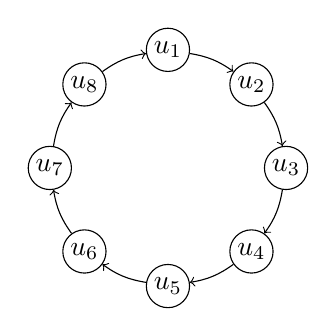
\begin{tikzpicture}[inner sep=0.5mm] 
\node[circle,draw] (u3) at (0:1.5) {$u_3$};
\node[circle,draw] (u2) at (45:1.5) {$u_2$};
\node[circle,draw] (u1) at (90:1.5) {$u_1$};
\node[circle,draw] (u8) at (135:1.5) {$u_8$};
\node[circle,draw] (u7) at (180:1.5) {$u_7$};
\node[circle,draw] (u6) at (225:1.5) {$u_6$};
\node[circle,draw] (u5) at (270:1.5) {$u_5$};
\node[circle,draw] (u4) at (315:1.5) {$u_4$};
\path (u1) edge [->,bend left=13] (u2);
\path (u2) edge [->,bend left=13] (u3);
\path (u3) edge [->,bend left=13] (u4);
\path (u4) edge [->,bend left=13] (u5);
\path (u5) edge [->,bend left=13] (u6);
\path (u6) edge [->,bend left=13] (u7);
\path (u7) edge [->,bend left=13] (u8);
\path (u8) edge [->,bend left=13] (u1);
\end{tikzpicture}
}\quad
\subfloat[][The 1st step]{\label{f2}
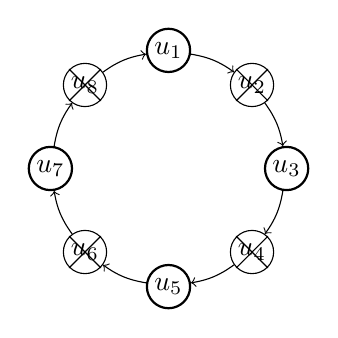
\begin{tikzpicture}[inner sep=0.5mm] 
\node[circle,draw,thick] (u3) at (0:1.5) {$u_3$};
\node[circle,draw] (u2) at (45:1.5) {$u_2$};
\node[circle,draw,thick] (u1) at (90:1.5) {$u_1$};
\node[circle,draw] (u8) at (135:1.5) {$u_8$};
\node[circle,draw,thick] (u7) at (180:1.5) {$u_7$};
\node[circle,draw] (u6) at (225:1.5) {$u_6$};
\node[circle,draw,thick] (u5) at (270:1.5) {$u_5$};
\node[circle,draw] (u4) at (315:1.5) {$u_4$};
\path (u1) edge [->,bend left=13] (u2);
\draw [line cap=round] (u2.north east) -- (u2.south west) (u2.north west) -- (u2.south east);
\path (u2) edge [->,bend left=13] (u3);
\path (u3) edge [->,bend left=13] (u4);
\draw [line cap=round] (u4.north east) -- (u4.south west) (u4.north west) -- (u4.south east);
\path (u4) edge [->,bend left=13] (u5);
\path (u5) edge [->,bend left=13] (u6);
\draw [line cap=round] (u6.north east) -- (u6.south west) (u6.north west) -- (u6.south east);
\path (u6) edge [->,bend left=13] (u7);
\path (u7) edge [->,bend left=13] (u8);
\draw [line cap=round] (u8.north east) -- (u8.south west) (u8.north west) -- (u8.south east);
\path (u8) edge [->,bend left=13] (u1);
\end{tikzpicture}
}\quad
\subfloat[][The 2nd step]{\label{f3}
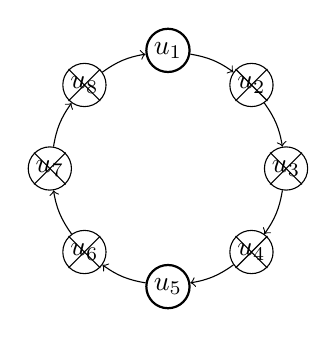
\begin{tikzpicture}[inner sep=0.5mm] 
\node[circle,draw] (u3) at (0:1.5) {$u_3$};
\node[circle,draw] (u2) at (45:1.5) {$u_2$};
\node[circle,draw,thick] (u1) at (90:1.5) {$u_1$};
\node[circle,draw] (u8) at (135:1.5) {$u_8$};
\node[circle,draw] (u7) at (180:1.5) {$u_7$};
\node[circle,draw] (u6) at (225:1.5) {$u_6$};
\node[circle,draw,thick] (u5) at (270:1.5) {$u_5$};
\node[circle,draw] (u4) at (315:1.5) {$u_4$};\path (u1) edge [->,bend left=13] (u2);
\draw [line cap=round] (u2.north east) -- (u2.south west) (u2.north west) -- (u2.south east);
\path (u2) edge [->,bend left=13] (u3);
\draw [line cap=round] (u3.north east) -- (u3.south west) (u3.north west) -- (u3.south east);
\path (u3) edge [->,bend left=13] (u4);
\draw [line cap=round] (u4.north east) -- (u4.south west) (u4.north west) -- (u4.south east);
\path (u4) edge [->,bend left=13] (u5);
\path (u5) edge [->,bend left=13] (u6);
\draw [line cap=round] (u6.north east) -- (u6.south west) (u6.north west) -- (u6.south east);
\path (u6) edge [->,bend left=13] (u7);
\draw [line cap=round] (u7.north east) -- (u7.south west) (u7.north west) -- (u7.south east);
\path (u7) edge [->,bend left=13] (u8);
\draw [line cap=round] (u8.north east) -- (u8.south west) (u8.north west) -- (u8.south east);
\path (u8) edge [->,bend left=13] (u1);
\end{tikzpicture}
}\quad
\subfloat[][The 3rd step]{\label{f4}
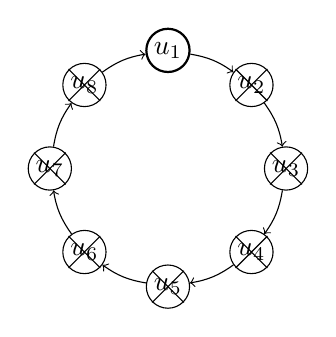
\begin{tikzpicture}[inner sep=0.5mm] 
\node[circle,draw] (u3) at (0:1.5) {$u_3$};
\node[circle,draw] (u2) at (45:1.5) {$u_2$};
\node[circle,draw,thick] (u1) at (90:1.5) {$u_1$};
\node[circle,draw] (u8) at (135:1.5) {$u_8$};
\node[circle,draw] (u7) at (180:1.5) {$u_7$};
\node[circle,draw] (u6) at (225:1.5) {$u_6$};
\node[circle,draw] (u5) at (270:1.5) {$u_5$};
\node[circle,draw] (u4) at (315:1.5) {$u_4$};
\path (u1) edge [->,bend left=13] (u2);
\draw [line cap=round] (u2.north east) -- (u2.south west) (u2.north west) -- (u2.south east);
\path (u2) edge [->,bend left=13] (u3);
\draw [line cap=round] (u3.north east) -- (u3.south west) (u3.north west) -- (u3.south east);
\path (u3) edge [->,bend left=13] (u4);
\draw [line cap=round] (u4.north east) -- (u4.south west) (u4.north west) -- (u4.south east);
\path (u4) edge [->,bend left=13] (u5);
\draw [line cap=round] (u5.north east) -- (u5.south west) (u5.north west) -- (u5.south east);
\path (u5) edge [->,bend left=13] (u6);
\draw [line cap=round] (u6.north east) -- (u6.south west) (u6.north west) -- (u6.south east);
\path (u6) edge [->,bend left=13] (u7);
\draw [line cap=round] (u7.north east) -- (u7.south west) (u7.north west) -- (u7.south east);
\path (u7) edge [->,bend left=13] (u8);
\draw [line cap=round] (u8.north east) -- (u8.south west) (u8.north west) -- (u8.south east);
\path (u8) edge [->,bend left=13] (u1);
\end{tikzpicture}
}
\caption{The case of $n=8$}\label{fig}
\end{figure}

As you can see, during the first step, $u_2,u_4,u_6$, and $u_8$ will be kill in order.
Then in the next step, $u_1$ kills $u_3$ and  $u_5$ kills $u_7$. These processes are depicted in Figures 
from~\ref{fig}.\subref{f1} to~\ref{fig}.\subref{f3} in sequence. Lastly, person no. 1 ($u_1$) kills person no. 5 ($u_5$); thus the last survival is $u_1$.
This is given in Figure~\ref{fig}.\subref{f4}.

\bigskip
Given the size of group $n$,  your mission is to find the index of person who finally survives in this game.
To do this, you should implement a C code which must \textbf{use a linked list} and \textbf{work recursively}.

\bigskip
\noindent\textbf{Input format.} %
The input is given a text-format file, named \texttt{input.txt} and all strings are separated by commas.
You should take as input the size integers $n$ with $i\geq 1$. 
\begin{lstlisting}[backgroundcolor=\color{yellow!40}]
n=$n$
\end{lstlisting}



\bigskip
\noindent\textbf{Output format.} %
The output should be given as a text-format file, named \texttt{outputc.txt}, \texttt{outputq.txt}, or \texttt{outputl.txt}.
The output file writes every survived person in each step following the format as described below.

\begin{lstlisting}[backgroundcolor=\color{yellow!40}]
$\ast\ast$ The initial step $\ast\ast$
$u_1 $ >> $u_2$ >> $\cdots$ >> $u_n$

$\ast\ast$ The 1st step $\ast\ast$
$u_{i_1}$ >> $u_{i_2}$ >> $\cdots$ >> $u_{i_k}$

$\ast\ast$ The 2nd step $\ast\ast$
$u_{j_1}$ >> $\cdots$ >> $u_{j_\ell}$
.
.
.
The last survival is person no. __
\end{lstlisting}
where all subscript numbers $i_1,\ldots,i_k,j_1,j_\ell\in\{1,\ldots,n\}$.

%\begin{figure}[h!]
%\centering
%\renewcommand{\thesubfigure}{d}
%
%\end{figure}
%
%\bigskip
%\noindent\textbf{Input format.} %
%The input is given a text-format file, named \texttt{input.txt} and all strings are separated by the blank character.
%\begin{lstlisting}
%$k$
%[$\delta_0$ $\delta_1$ $\cdots$ $\delta_k$]
%$\ell$
%[$f_{1,0}\ f_{1,1}\ f_{1,2}\ \cdots\ f_{1,n_1}$] 
%[$f_{2,0}\ f_{2,1}\ f_{2,2}\ \cdots\ f_{2,n_2}$]
%	$\vdots$
%[$f_{\ell,0}\ f_{\ell,1}\ f_{\ell,2}\ \cdots\ f_{\ell,n_\ell}$]
%[$g_{1,0}\ g_{1,1}\ g_{1,2}\ \cdots\ g_{1,m_1}$]
%[$g_{2,0}\ g_{2,1}\ g_{2,2}\ \cdots\ g_{2,m_2}$]
%	$\vdots$
%[$g_{\ell,0}\ g_{\ell,1}\ g_{\ell,2}\ \cdots\ g_{\ell,m_\ell}$]
%\end{lstlisting}
%where $k$ is the degree of your chosen irreducible polynomial $\delta(x)=\delta_kx^k+\delta_{k-1}x^{k-1}+\cdots+\delta_1x+\delta_0$  
%which is given at the second line and $\ell$ is the number of target polynomials. 
%For some $1\leq i\leq \ell$, the $\ell$ polynomials from the 4-th line states  $F_i(x)=\displaystyle\sum_{j=0}^{n_i}f_{i,j}x^j$ of degree $n_i$ with each $0\leq n_i\leq k$,
%the next $\ell$ polynomials to the last line states $G_i(x)=\displaystyle\sum_{j=0}^{m_i}g_{i,j}x^j$ of degree $m_i$ with each $0\leq m_i\leq k$.
%
%You should randomly generate $2\ell$ polynomials $F_1(x),\ldots,F_\ell(x),G_1(X),\ldots,G_\ell(x)$.
%
%\bigskip
%\noindent\textbf{Output format.} %
%The output should be given as a text-format file, named \texttt{output.txt}. For every $1\leq i\leq \ell$,
%the output file writes all resulting polynomials $R_i(x)=\displaystyle\sum_{j=0}^{v_i}r_{i,j}x^j$ of division between target polynomials so that $R_i(x)=F_i(x)\boxdiv G_i(x)$
%in the form of vector.
%\begin{lstlisting}
%[$r_{1,0}\ r_{1,1}\ r_{1,2}\ \cdots\ r_{1,v_1}$]
%[$r_{2,0}\ r_{2,1}\ r_{2,2}\ \cdots\ r_{2,v_2}$]
%	$\vdots$
%[$r_{\ell,0}\ r_{\ell,1}\ r_{\ell,2}\ \cdots\ r_{\ell,v_\ell}$]	
%\end{lstlisting}



%\section*{Background}
%
%Let $\Z$ be the set of the integers.
%Doing arithmetic over $\Z$, there are two critical problems: (1) because $\Z$ is infinite, we cannot 
%express the set $\Z$ on any computing machine, and (2) because $a\div b\notin\Z$ for some integers $a,b\in\Z$, division over $\Z$ is not closed.
%For example, when $a=1,b=2$, it is clear that $1\div 2\not\in\Z$.
%
%To solve these problems, we build the set $\Z_p=\{0,1,\ldots,p-1\}$  for a positive integer $p>1$.
%It is well known that for all integers $a,p\in\Z$ with $p>0$,
%there exist unique $q,r$ such that $a=pq+r$ and $0\leq r<p$.
%Using the theorem, let us define a  function $\md(\cdot,\cdot)$ as follows.
%\begin{equation*}
%\md(a,p) := a\pmod{p} = r.
%\end{equation*}
%Next, we define four basic operations in $\Z_p$ for an integer $p>2$. For all $a,b\in\Z_p,$
%\begin{equation*}
%\begin{array}{rcl}
%a\boxplus b &:=& (a+b)\pmod{p}=\md(a+b,p),\\
%a\boxminus b &:=& (a+(p-b))\pmod{p}=\md(a+(p-b),p),\\
%a\boxdot b &:=& (a\cdot b)\pmod{p}=\md(a\cdot b,p),\\
%a \boxdiv b &:=& (a\cdot b^{-1})\pmod{p}=\md(a\cdot b^{-1},p)\\
%\end{array}
%\end{equation*}
%where $b^{-1}$ is the multiplicative inverse of $b$ modular $p$; in other words, $1=\md(b\cdot b^{-1},p)$.
%According to Euler's theorem, when $p$ is a prime, for all non-zero $b\in\Z_p$ there always exists unique $\beta\in\Z_p$  
%such that $\md(b\cdot \beta,p)=1$. In fact, we can find such a multiplicative inverse $\beta=b^{-1}\mod p$ of $b\in\Z_p$
%using the \emph{extended Euclidean algorithm} (EEA). 
%Because $b,\beta\in\Z_p$ and multiplication is closed in $\Z_p$, 
%It is easy to check that $a\boxdiv b=c\in\Z_p$.
%
%\medskip
%Consider the set $\Z_p[x]$ which consists of  all polynomials $f(x)=f_0+f_1x+\cdots+f_nx^n$  whose coefficients are in $\Z_p$. 
%Then we will meet the same problems in doing arithmetics over $\Z_p[x]$ as calculating over $\Z$.  
%Similarly, we see that $\Z_p[x]$ is an infinite set because the degree of $f(x)\in\Z_p[x]$  is not fixed.
%Moreover, because $f(x)\div g(x)\notin\Z_p[x]$, polynomial division is not closed in $\Z_p[x]$.
%To fix these problems, we introduce an irreducible polynomial $\delta(x)=\sum_{i=0}^k\delta_ix^i$ with $\delta_k=1$ for a fixed integer $k>1$.
%You may think of the irreducible polynomial $\delta(x)$ as a prime number $p$ in $\Z_p$.
%Given a prime number $p$ and an irreducible polynomial $\delta(x)\in\Z_p[x]$ of degree $k$, 
%we can construct a finite set of polynomials $\Z_p[x]/\langle\delta(x)\rangle =\{f(x)|f(x)=f_0+f_1x+\cdots+f_{k-1}x^{k-1}\text{ for each }f_i\in\Z_p\}$.
%That is to say, $\Z_p[x]/\langle\delta(x)\rangle$ is the set of all polynomials whose degree  $<k$ and coefficients are in $\Z_p$.
%
%\medskip
%Now we can can compute polynomial arithmetic over  $\Z_p[x]/\langle\delta(x)\rangle$ as follows. Let $f(x),g(x)\in\Z_p[x]/\langle\delta(x)\rangle$ and they are written by
%$f(x)=\displaystyle\sum_{i=0}^nf_ix^i,g(x)=\sum_{i=0}^m g_ix^i$ for  integers $0\leq n,m<k$ and 
%with $f_n\neq 0,g_m\neq 0$. Assuming that $n\geq m$, we have 
%\begin{eqnarray*}
%f(x)\boxplus g(x) &:=&\sum_{i=0}^n\md(f_i+g_i,p)x^i,\\
%f(x)\boxminus g(x) &:=&\sum_{i=0}^n\md(f_i+(p-g_i),p)x^i,\\
%f(x)\boxdot g(x) &:=&\md\left(\sum_{i=0}^{n+m} \left(\sum_{j=0}^{i} f_j\boxdot g_{i-j}\right)x^i,\delta(x)\right)
%	=\md\left(\sum_{i=0}^{n+m}\md\left(\sum_{j=0}^{i} f_j\cdot g_{i-j},p\right)x^i,\delta(x)\right),\\
%f(x)\boxdiv g(x) &:=& f(x)\boxdot g(x)^{-1}
%\end{eqnarray*}
%where $g(x)^{-1}$ is the multiplicative inverse polynomial of $g(x)$ modular $\delta(x)$; in other words,
%$1=g(x)\boxdot g(x)^{-1}$.
%
%
%For example, consider a setting where $p=3$ and $\delta(x)=x^3+2x+1$. Let $f(x)=2x^2+x,g(x)=x^2+2$.
%Then $f(x)\boxplus g(x)=2x^2+x+x^2+2=3x^2+x+3=x$ and $f(x)-g(x)=2x^2+x-x^2-2=x^2+x-2=x^2+x+1$. 
%We have
%\begin{eqnarray*}
%f(x)\boxdot g(x) &=& (2x^2+x)\boxdot (x^2+2)=2 x^4 + x^3 + 4 x^2 + 2 x\mod\delta(x) \\
%		&=& x+2\\
%\end{eqnarray*}
%and
%\begin{eqnarray*}
%f(x)\boxdiv g(x) &=& (2x^2+x)\boxdot(x^2+2)^{-1}\\
%			&=&(2x^2+x)\boxdot 2x\\
%			&=&4x^3+2x^2\mod\delta(x)=x^3+2x^2\mod\delta(x)\\
%				&=& 2x^2-2x-1=2x^2+x+2.
%\end{eqnarray*}
%Similarly, we can find the multiplicative inverse of $g(x)$ modular $\delta(x)$ over $\Z_p[x]/\langle\delta(x)\rangle$,
%using the EEA. See the below how the EEA runs over $\Z$.


\newpage
\begin{thebibliography}{100}
%\addtolength{\leftmargin}{0.2in}
%\setlength{\itemindent}{-0.2in}

\bibitem[GT15]{GT15} M. Goodrich and  R. Tamassia, \emph{Algorithm design and applications}, Wiley. 


\bibitem[Jos27]{Jos27}  Flavius Josephus, \emph{The jewish war  Book III},  Translated by H. S. Thackeray,  Heinemann 1927,
342--366 \& 387--391.
 \end{thebibliography}            
\end{document}

 


































